\section{Introduction}

Image-based modeling and simulation is becoming an increasingly important analytic and predictive tool for a variety of medical and engineering applications. Some examples include patient-specific diagnosis and treatment, large-scale \textit{in silico} trials, medical device design, computer-assisted surgery, and analysis of as-built structures and components. Image-based modeling and simulation comprises a long chain of methodological elements, which we organize into several major task domains:  
\begin{enumerate}
\item
segmentation of the raw image, 
\item
creation of a boundary representation (b-rep) of the problem domain,
\item
generation of a suitable volume mesh (finite elements or other), 
\item
assignment
of boundary conditions and constitutive models, and finally 
\item
the physics-based
simulation itself on the volume mesh.
\end{enumerate}

This article focuses on the second of these task domains:  creation of a b-rep given a segmented image (i.e. an image mask).  
This single step in the overall 
image-to-analysis pipeline itself typically consists of several sub-steps.  
We describe our approach alongside three alternatives, and offer both quantitative and visual comparisons.  We use the term {\em b-rep} instead of {\em surface}
in order to emphasize certain properties that are essential to the target
application:  namely, the b-rep must be closed and oriented (and therefore
``watertight''), and manifold in the case of only a single material domain
(as is our present focus).  We further stipulate that the b-rep should consist of
an assemblage of simple polygonal facets defined by shared vertices and 
edges.  In view of the present application, the b-rep creation method should engender a degree of
flexibility in the geometry of the facets, in order to accommodate the subsequent
volume-meshing step.  Specifically, the finite elements of the
volume mesh, which are typically many times larger than the
voxel grid size, must register with the b-rep's facets.

Our overarching objective is to
achieve a high degree of automation in the overall image-to-analysis process.
We therefore place particular emphasis on 
computational {\em robustness}:  given a segmented image that is in some sense
noisy, our goal is that the b-rep should nevertheless ultimately support
the generation of a computable volume mesh.  In rough terms, if the
image mask is good enough to define a sensible problem domain, the resulting
b-rep should reliably exhibit suitable water-tightness
and topological-correctness properties.  

Our method of b-rep extraction relies on two 



Given the present goal of supporting robust image-to-analysis processes, it 
seems appropriate to digress briefly to describe the particular demands 
on the image-to-b-rep step in this setting.  Those 
demands turn, to a great degree, on the specifics of the subsequent
volumetric meshing.  In most practical circumstances, the final volumetric mesh
must be much less dense than the voxel grid, such that some form of coarsening, or {\em decimation}, of the b-rep is necessary.   If automatic tetrahedral or mixed tet/hex meshing is to be used, then the b-rep and the volumetric mesh must ultimately
align with each other at the surface of the problem domain.  
Tetrahedral meshing is the natural choice for meshing volumes bounded by triangulated b-reps.  The two most widely adopted approaches for automated unstructured tetrahedral mesh generation are \textit{advancing front}~\cite{jin_1993, lohner_1988} and \textit{Delaunay tetrahedralization}~\cite{lohner_1997}.


 Updegrove \textit{et al.}~\cite{updegrove_2016} used a \textit{lofting} technique on a series of 2D segmentations to generate models of blood vessels. In lofting, an approximate centerline is drawn, and 2D segmentations are combined using spline interpolating functions to generate surfaces. Unstructured tetrahedral meshes are then generated from the surfaces. Lofting is known as a 2.5D approach because stacked contours of neighboring slices cannot capture arbitrary 3D topologies. The interpolating splines typically require manual selection of control points~\cite{young_2008}. Treating an image mask as a series of 2D masks was a popular approach in past decades, More recent approaches treat the mask as a three-dimensional object to avoid the limitations of lofting techniques.
 
 Young \textit{et al.}~\cite{young_2008} used a \textit{direct meshing} approach to generate meshes from multi-material image masks, without the intermediate step of creating a surface mesh. Young \textit{et al.} combined the surface generation and mesh generation stages into one process via their \textit{enhanced volumetric marching cubes} approach. Rather than simply determining triangular surface patches from the intersection of the isosurface with grid cells, volumetric marching cubes generates tetrahedral volumes directly. The authors extended their volumetric algorithm to handle intersections of up to eight regions in one grid cell -- the maximum number of intersections that can occur for a Cartesian grid. The resulting mesh is \textit{mixed hex-tet}, where tetrahedra exist near the surface based on the extended volumetric marching cubes approach; internal voxels are converted directly to hexahedra; and pyramidal and tetrahedral elements exist in the transitional layer in between. The authors also utilized partial volume-based interpolation to improve surface smoothness. Additional efforts to reduce the mesh size were made by converting surface tetrahedra to hexahedra where appropriate, and by performing an octree-based approach to collect neighboring interior hexahedral elements into larger elements. Nonetheless, this \textit{grid-based} approach results in a surface mesh that is very fine, which subsequently constrains the size of interior elements in the volume mesh. The resulting mesh from this approach yields a large number of degrees of freedom for simulation purposes. Thus, for practical purposes, the number of points and polyhedra defining the surface must be reduced, or \textit{decimated}, to allow for a subsequent coarser volumetric discretization. Indeed, the default and recommended approach in their software \textit{Simpleware} (known as \textit{+FE Free}) is to follow the two-step paradigm of surface generation followed by CAD-based meshing as described previously. Namely, the software extracts the resulting surface from the extended volumetric marching cubes step, performs multi-part decimation and smoothing~\cite{egst}, and finally uses a conventional CAD-based tetrahedral mesher to generate fully tetrahedral meshes from the polygonized surfaces.

\begin{figure}[t]
	\centering
		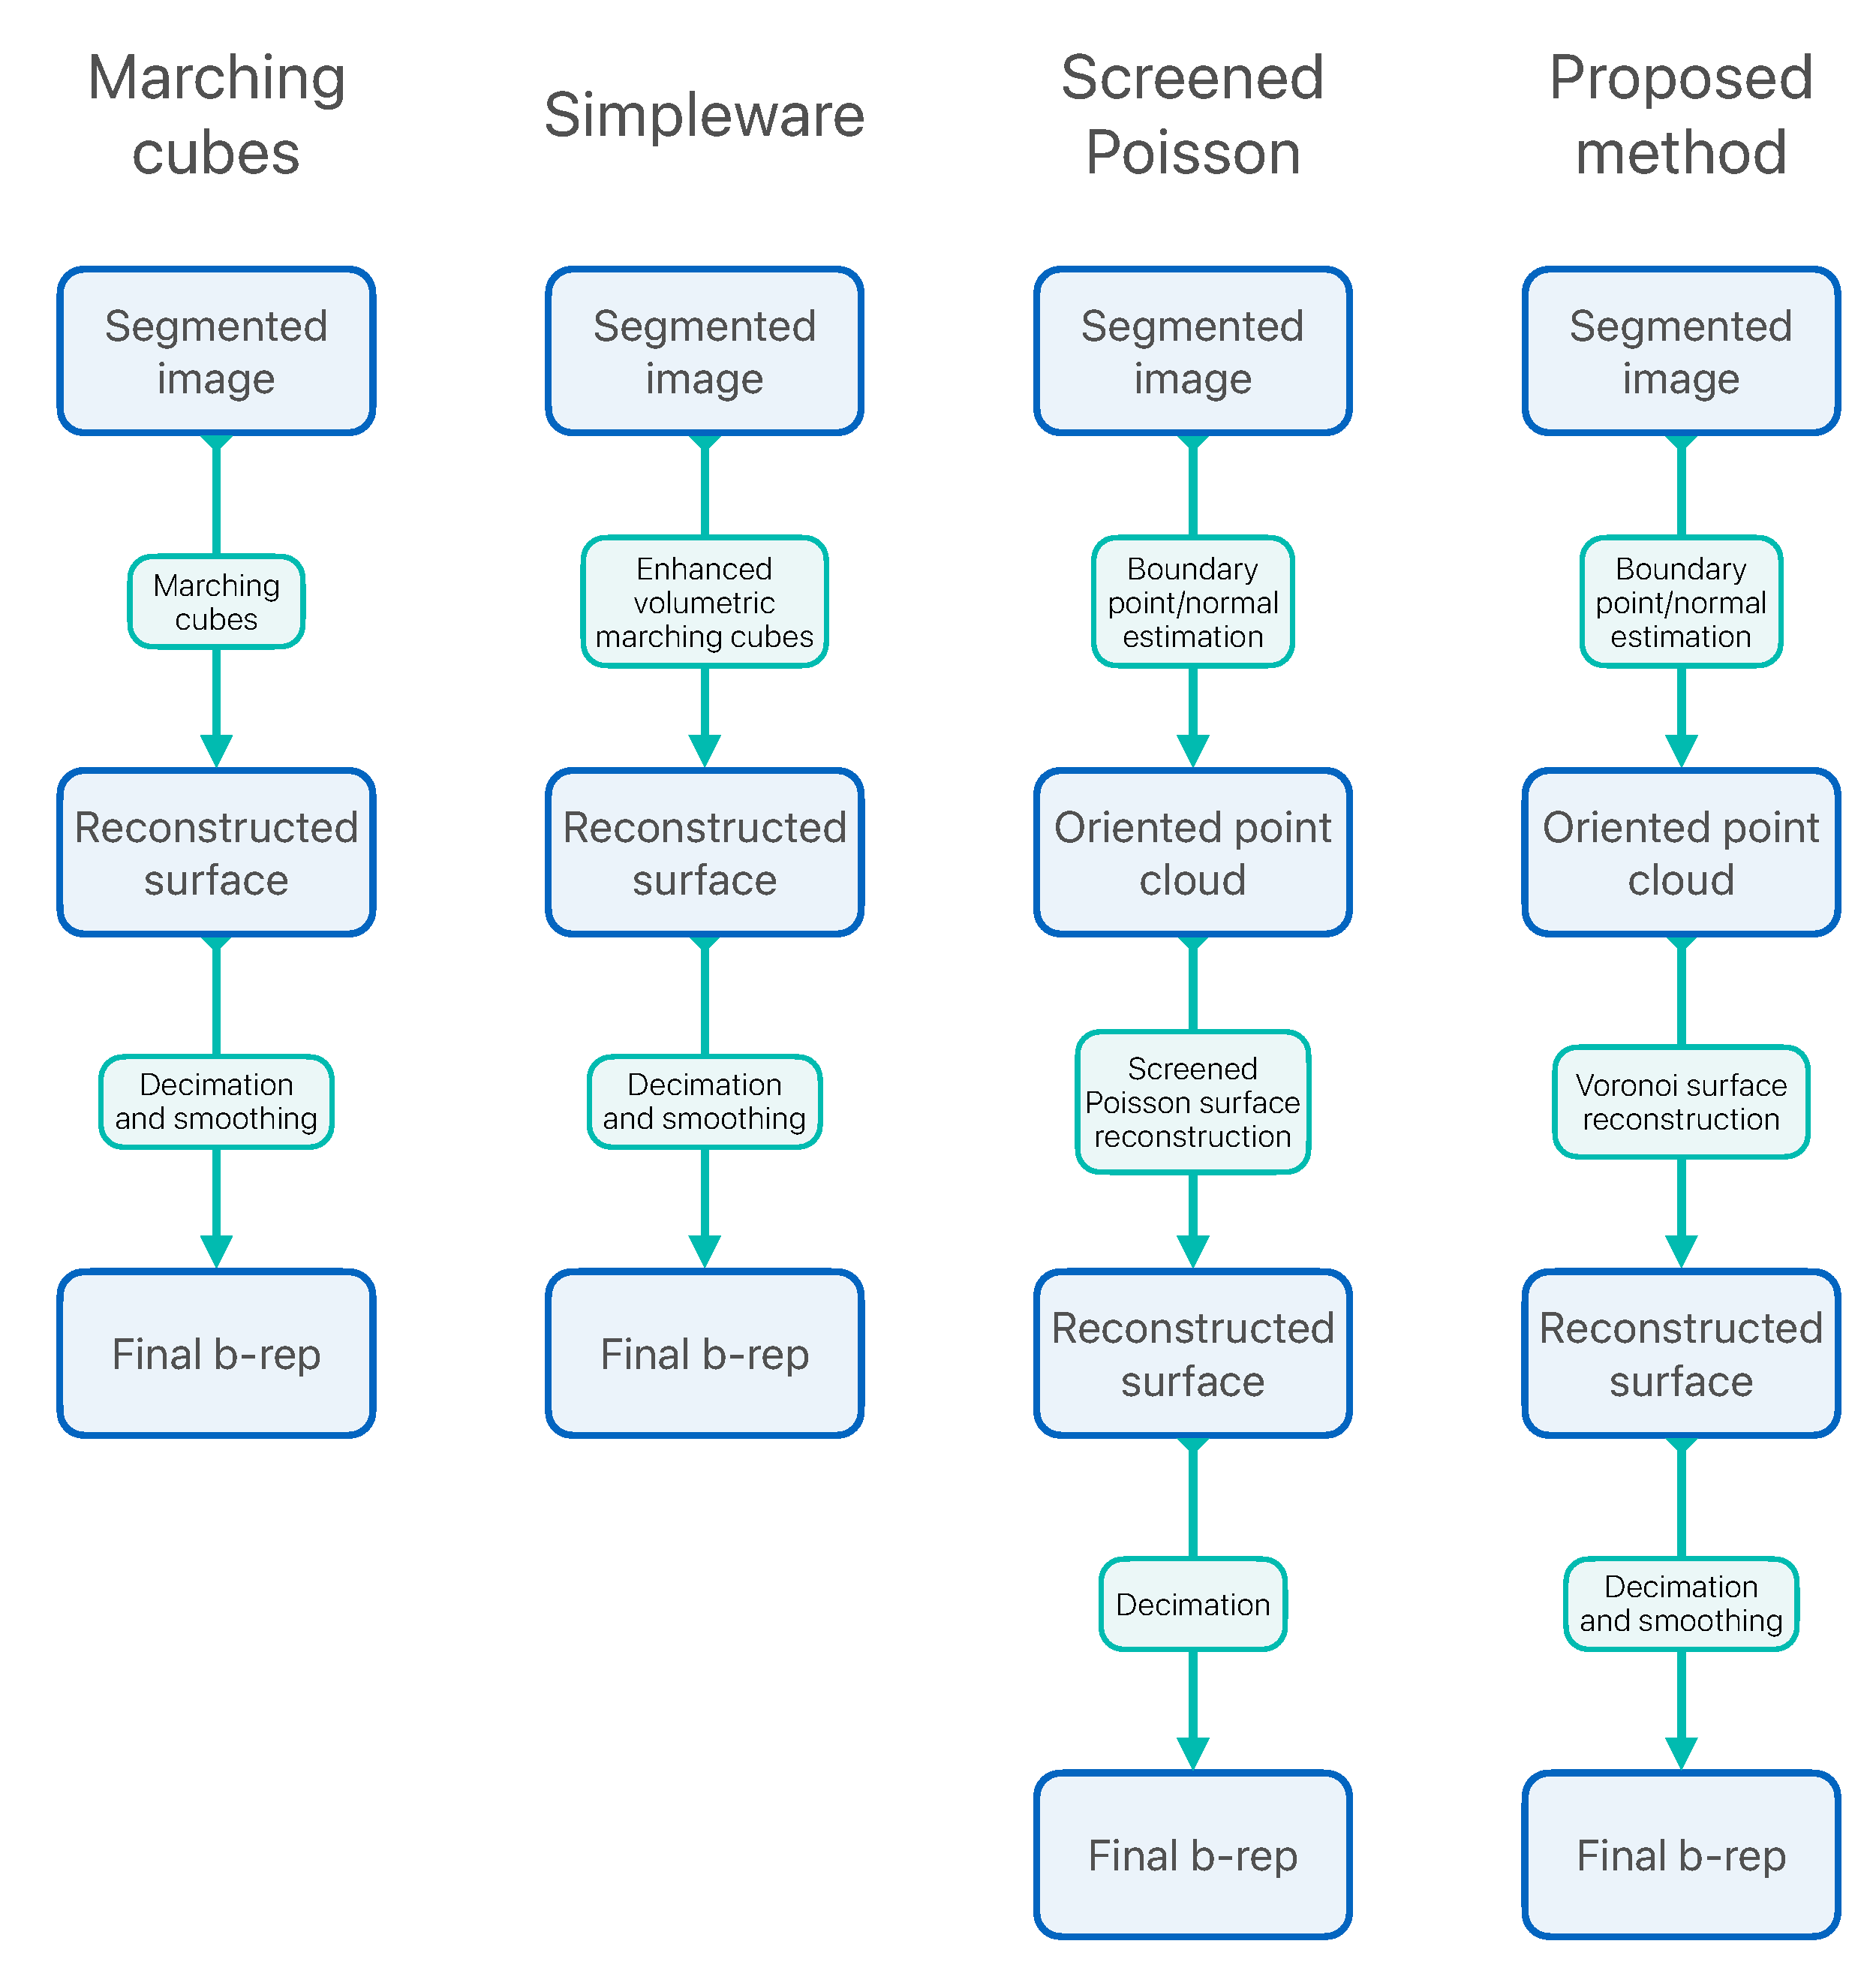
\includegraphics[scale=0.3]{media/flowchartNew.pdf}
	\caption{Flowcharts of different techniques to generate b-reps from image masks.}
	\label{fig:flowchart}
\end{figure}\noindent

%
Medical imaging is the process of generating discrete image representations of the regions of interest. For the present purposes, the acquired image provides a three-dimensional rectilinear grid of point intensity values as input to the rest of the workflow. In the case of MRI, these values are weighted proton densities, which effectively measure water content. In the case of CT, they are attenuation measurements from an x-ray beam source, which effectively measure density. For typical applications, we can expect millimeter resolution, and in some cases considerably better~\cite{van2012super}.\\ \\
%
Image segmentation is the process of partitioning an image into non-overlapping regions corresponding to different tissues or objects in an image. Contrast differences between neighboring tissues can be difficult to identify due in part to noise and artifacts. Thus, image processing in the form of smoothing, filtering, and resampling are performed to improve the effectiveness of the image segmentation technique. The output from image segmentation consists of \textit{image masks} defining each of the regions of interest in the field of view. If there is only one region of interest, the output is termed a \textit{binary image mask}. Some popular image segmentation techniques include thresholding, level set methods~\cite{malladi_1995, sethian_1996}, and machine-learning-based approaches~\cite{litjens_2017}.  For practical purposes, manual fine-tuning is typically required for any of these methods.\\ \\



Many image-based volumetric meshing approaches rely on the \textit{marching cubes} algorithm~\cite{lorensen_1987} and its variants. Marching cubes assumes the existence of an implicit isosurface, which can be defined on the voxel grid taken as a structured hex mesh.  Triangular patches are generated to approximate the intersection of this isosurface with each grid cell; the triangles are then connected together to form a continuous surface. B-reps generated via marching cubes generally exhibit fairly strong aliasing, and the algorithm in its standard form is applicable only to binary image masks, i.e. those that contemplate only a single material type.  Advances in the field of image-based meshing have largely focused on modifications to the standard marching cubes algorithm to address these two limitations, namely: 1) generating smooth surfaces that represent the original object accurately while preserving sharp features; and 2) generating quality surface meshes for general multi-material image masks (cite refs here).

Meyer \textit{et al.}~\cite{meyer_2008} employed a \textit{particle-based sampling} technique for multi-material volumes. Surface samples (called \textit{particles}) are constrained to the zero set of an implicit function. The distances between particles are locally adapted to create higher densities of points near surface features. A Delaunay tetrahedralization of the sampling points is computed, and each tetrahedron is assigned a material label. The surface mesh is generated by extracting the faces bounded by tetrahedra with different material labels. Finally, a conventional CAD-based tetrahedral mesher is employed to produce an analysis-ready mesh. The approach faithfully and robustly captures the geometries of complex material interfaces. However, the authors report long run times.
Examples of other image-based meshing techniques include \cite{fang_2009, mohamed_2004, jermyn_2013, boissonnat_2009}. 

Recently, many authors have turned their attention to surface generation from multi-material image masks. However, generation of high-quality surfaces, and subsequently volume meshes, from binary image masks remains a challenge and a fertile area of research. This will be the focus of the present paper.  We propose a novel Voronoi-based surface generation approach that guarantees watertightness and constitutes a framework that can readily be extended to encompass sharp boundary features and multi-material domains. The method is simple to use in terms of human effort and is generally free of adjustable parameters that need to be tuned to obtain desirable results. \\ \\
%
Finally, provided a triangulated surface mesh from any of the aforementioned approaches, conventional CAD-based volume-meshing techniques can be utilized to produce a volume mesh. If a volume mesh is desired, tetrahedral meshing is usually the method of choice for meshing arbitrary triangulated boundary surfaces. The two most widely adopted approaches for automated unstructured tetrahedral mesh generation are \textit{advancing front}~\cite{jin_1993, lohner_1988} and \textit{Delaunay tetrahedralization}~\cite{lohner_1997}. \\ \\
%
Applications for this work span across 3D printing, visualization, and finite element analysis (FEA). In the case of 3D printing and visualization, b-reps can be used for surgery planning, custom surgical guides and implants, rapid prototyping, and generation of CAD surfaces from existing parts. Meanwhile, image-based simulation has been performed on nearly every major organ in the body and shows great promise in advancing both personalized medicine~\cite{neal2010current} and large-scale clinical trials~\cite{viceconti2016silico}. In addition, image-based simulation offers the ability to perform non-destructive analysis on as-built engineering parts or legacy parts where CAD data may not be available~\cite{bradley2005advances}.\\ \\
%
Provided the context of the image-based modeling workflow, we present our Voronoi-based surface generation algorithm in the next section. A performance assessment follows, which includes comparison to \textcolor{purple}{other approaches}.  We consider both quantitative error measures as well as qualitative, visual comparison of b-rep results.  The paper is closed with a summary and discussion of future directions for this work.

\textcolor{purple}{
Notes from Omar:\\
- When discussing marching cubes/aliasing, we need to acknowledge that our proposed method also exhibits aliasing. But as will be demonstrated in the performance assessment section, to a much lesser degree\\
- Addressing the reviewer comment about our method not being able to handle sparse point clouds - maybe a quick comment somewhere along the lines of: The intention of our method is to produce a dense point cloud from fairly low-resolution image data. By definition, our method produces dense point clouds. So the scope of our surface reconstruction step is as such. And addressing sparse point clouds is out of our scope.\\
- Reviewer comment emphasizing for us to mention moving least squares and this Fleishman reference~\cite{fleishman2005}. ``When discussing the point cloud => mesh step, it seems to me that moving least\\
squares approaches should be mentionned. For instance "Robust Moving Least
Squares Fitting With Sharp Features" by Fleishman et al.''\\
- At some point around us discussing the flowchart, we need to explain why we do not perform smoothing for the Poisson approach. The reason is that screened Poisson surface reconstruction already performs smoothing on the indicator function in its algorithm. In fact, the paper touts ``We also observe that the screened Poisson reconstruction introduces less smoothing, providing a reconstruction that is truer to the original data than either the original Poisson or the SSD reconstructions''. The counter would be that the decimation step introduces error. However, we checked this and decimation does not significantly impact our error measures in the Performance Assessment section. All that said, we did try adding Taubin smoothing to the Poisson results as a last step, and the results are still similar to the proposed method, with the proposed method still performing slightly better for the sphere.
- several of the reviewer comments about other work probably belong here in the introduction rather than in the Limitations section
- both reviewers seemed to think we ``discarded'' Poisson surface reconstruction after mentioning it. Let's be sure not to sound dismissive about it or other methods}